\documentclass{scrartcl}

\usepackage{tikz}
\usetikzlibrary{shapes,arrows,positioning}

\tikzstyle{decision} = [diamond, draw, fill=blue!20, text width=4.5em, text badly centered, node distance=3cm, inner sep=0pt,on grid]
\tikzstyle{block} = [rectangle, draw, fill=blue!20, text width=5em, text centered, rounded corners, minimum height=4em,on grid]
\tikzstyle{line} = [draw, -latex]

\begin{document}

  \begin{center}
    \resizebox{0.4 \linewidth}{!}{%
      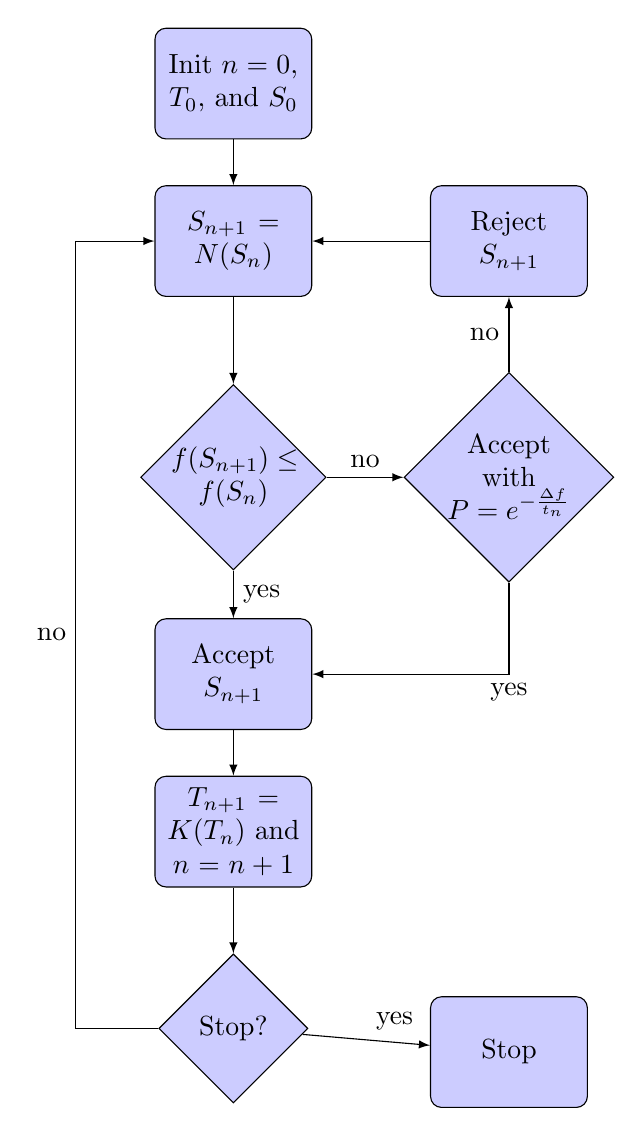
\begin{tikzpicture}[node distance = 2cm, auto]
        \node[block]                                (init) {Init $n=0$, $T_0$, and $S_0$};
        \node[block, below= of init]                (nbrh) {$S_{n+1}=N(S_n)$};
        \node[decision, below= of nbrh]             (ovgt) {$f(S_{n+1}) \le f(S_n)$};
        \node[block, below=2.5cm of ovgt]           (accp) {Accept $S_{n+1}$};
        \node[decision, right= 3.5cm of ovgt]       (rand) {Accept with $P = e^{-\frac{\Delta f}{t_n}}$};
        \node[block, above=3cm of rand]             (rejj) {Reject $S_{n+1}$};
        \node[block, below= of accp]                (incr) {$T_{n+1} = K(T_n)$ and $n=n+1$};
        \node[decision, below=2.5cm of incr]              (stcd) {Stop?};  
        \node[block, right=3.5cm of stcd, yshift=-3mm]                (stop) {Stop};


        \path[line] (init) --          (nbrh);
        \path[line] (nbrh) --          (ovgt);
        \path[line] (ovgt) -- node{yes}(accp);
        \path[line] (ovgt) -- node{no} (rand);
        \path[line] (rand) -- node{no} (rejj);
        \path[line] (rejj) --          (nbrh);
        \path[line] (rand) |- node{yes}(accp);
        \path[line] (accp) --          (incr);
        \path[line] (incr) --          (stcd);
        \path[line] (stcd) -- node{yes}(stop);
        \path[line] (stcd) -- ++(-2,0) |- node[pos=.25]{no}  (nbrh);
      \end{tikzpicture}%
    }%
  \end{center}


\end{document}
